\chapter{系统实现}

\section{诊断算法}
诊断算法:从上海中医药大学龙华医院、曙光医院、上海瑞金医院以及上海本地的十余家医院和社区中,采集了15万分样本数据作为训练数据和测试数据,处理流程包括图片预处理,面部舌部特征提取,使用分类器进行分类等。

问诊问题是根据《八纲》和《体质辨证理论设计问诊量表》经过专家论证,结合用户测试反馈,经过反复 11 次讨论和相关专家论证,最后确定了最有指向性的12个问题作为问诊内容。新版问题:遵循传统中医的问诊规律,除年龄、性别、体重等常规性提问外,还设13个现状性问题,主问寒热、汗、头身、胸胁、胃脘、腰腹、饮食、睡眠、情志、二便,并针对女性、小儿、老人增设附加问题;

照片预处理的目的主要是要通过色彩校正和图像质量优化获得符合计算机检测要求的标准图像;

面部特征提取需要计算人脸的光泽程度,将人脸的光泽程度划分为有光泽,少光泽无光泽等,同时将嘴唇形状,嘴唇位置等信息作为先验条件,对上半脸进行高斯建模完成分割唇部作为特征;

舌部特征提取主要是完成舌质颜色,舌苔颜色,舌苔厚薄,舌裂纹,舌胖瘦,舌齿印等特征;

特征验证方面,15 名中医临床专家对81张患者开放环境下舌象图片进行了判读,次日同一时间将舌象图片重新随机编号,5 名中医专家再次进行判读。对每个中医专家的两次判读结果进行分析,总一致率基本在80\%以上。这些检验证实各量表可信度较高,可满足软件设计需求;

特征分类器使用了高斯混合模型,支持向量机和前馈神经网络完成,诊断算法是由上海中医药大学的专业医生编写的一个规则系统,最后把人的体质归为阳虚,阴虚,痰湿,淤滞,脾虚,肾虚,气虚,正常几类,并通过回答的问题和面部舌部的得分,对于每个用户给出一个健康分数和对应的养生建议;

最后给出的养生建议包括“环境起居”、“中医功法”、“情志调适”、“音乐调摄”、“食疗药膳”、“穴位保健”等几个方面帮助用户更好地调理健康。

\subsection{算法流程}
我们使用云中医的算法作为系统的诊断算法。

\begin{figure}
    \centering
    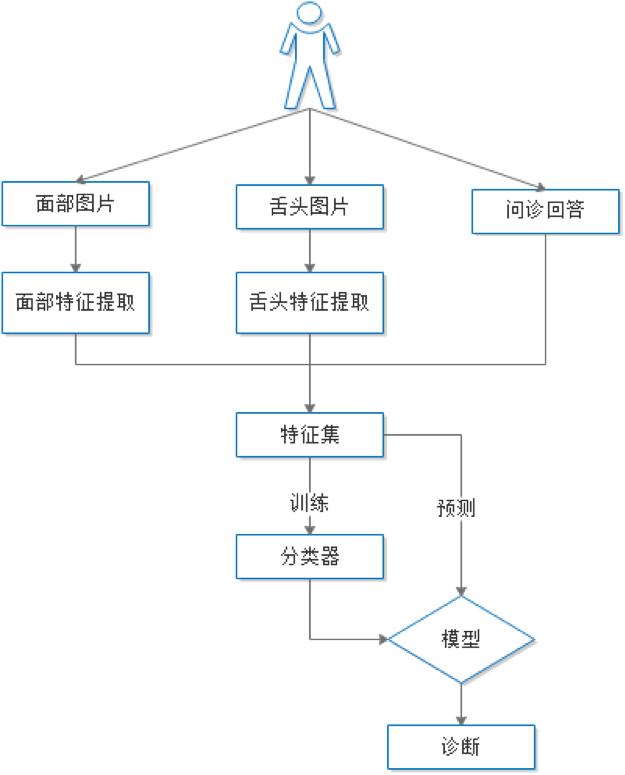
\includegraphics{images/1.png}
    \caption{图片处理流程}
    \label{fig:f1}
\end{figure}

\subsection{输出结果}



\section{服务端实现}
为了能够满足系统的跨平台使用,我们需要把诊断算法从客户端剥离到服务器,通过接口调用的方式来实现面诊和舌诊。

服务端提供了以下几个功能:
保存用户操作日志,返回面诊舌诊结果,保存用户信息以及诊断记录。



\section{客户端实现}
设计新的自诊界面,解决交互方面易用性的问题,给用户对自己当前状态一种直观的感受。
 
如图所示,根据用户调研的反馈,新界面简化了诊断的流程,面诊舌诊问诊在一个页面显示,并且所有的问题和操作都是可选的,不会出现必须要先面诊然后舌诊然后才能问诊的问题。其次,新界面对面诊和舌诊进行了中间结果的反馈,面诊在用户拍照确认之后,会立即报告本次照片是否合格已经诊断的结果,用户不需要在点击诊断的时候才被提示照片不合格。
在问诊方面,新系统实现了最近一次记录保存,由于问题是可选回答的,所以用户只需要回答和自己上次的结果不一致的即可。同时,我们对不同问题的回答结果进行了颜色的区分。有色实心代表本次回答,有色空心代表上次回答;橙色代表有症状,绿色代表回答的问题表现良好,没有症状;白色没有填充和边框,为黑字,代表未回答。
在方框内部的问题描述设计上,我们把默认的文字描述,显示为问题描述;一旦用户本次或者上次回答过该问题,则直接显示用户回答的结果。这样做的结果是,第二次用户点进来,就能看到上次的回答结果,这样能够对自己的身体情况有个快速的了解。
跨平台应用实现方面,系统界面采用mui框架,界面交互使用angular及其插件完成,复杂计算和逻辑通过后台调用实现,系统主要有以下几个模块:
用户登录模块:
 
用户登录时,需要输入正确的手机号才能通过手机格式验证发送验证码到手机上。
 
系统首页:
 
首页简化之后,只保留了新版和旧版界面的入口,方便用户进行对比,同时,用户也可以在首页下面的tab页查看自己之前的诊断记录。
诊断界面:
 
	新界面和之前版本的云中医界面不同的是,诊断界面不仅提供了面诊舌诊问诊的入口,同时会将面诊舌诊的照片和中间结果直接显示在当前页面,给用户对于自己当前身体情况一个直观的感受。如果拍照失败会直接显示,不需要等到用户进行点击诊断之后才知道自己的照片不合格。
面诊舌诊:
 
用户通过点击面诊或者舌诊的圆圈图案,可以通过从相册选择或者通过拍照,上传自己的脸部或者舌头照片。图片裁剪可以帮助用户定位面部和舌头的位置,提高诊断的精度。用户点击确认裁剪之后,诊断的结果会直接显示在圆圈下面,同时,如果没有识别到人脸或者舌头也会提示用户重新拍照。点击确认裁剪后,通过对图片进行base64编码上传到服务器的诊断接口拿到诊断结果。
问诊:
 
问诊的问题一共13道,用户根据自己的情况通过勾选回答问题。每次进入问诊界面,系统会尝试加载上一次用户回答问题的历史记录和对应的答案。同时,回答过的问题,会在界面上进行显示。没有回答过的问题,将是白色黑字没有边框。
诊断:


用户在完成自己需要回答的问题或者面诊舌诊之后,可以点击蓝色的诊断按钮进行健康诊断,同时,系统会将本地诊断记录上传到后台服务器上,以便查询诊断记录。

诊断结果:
 
系统根据用户个人的情况,会给出面诊结果,舌诊结果和最后的体质以及健康分数。此外,根据体质的不同,会给出和体质对应的健康建议,帮助用户进行针对性的健康调理。

诊断记录列表:
 
诊断记录页面,能够直观地给出用户近期的健康变化的情况。用户可以点击诊断记录,进入当时的详细诊断结果页面。